\chapter{Electric and Chromo-electric Dipole Moment of Quarks}
\label{ch:quark(C)EDM}

After the analysis for leptons, we turn our gaze towards EDMs involving quarks. 
As mentioned in the theory section, there are additional chromo-EDM and Weinberg term contributions to take into account that arise from the fact that quarks interact via QCD.
However, since quarks are always confined as hadrons, it is extremely difficult, if not outright impossible, 
to directly probe the EDMs of individual quarks, given the state of current technology and our understanding of QCD.
A quick literature~\cite{PDG2022} review shows that there are indeed no direct experimental observations for the EDMs of all the quarks lighter than the top quark.
We comment on the situation of the top quark in \secref{top-cedm}. 
It is natural, under these circumstances, to shift our attention towards hadron EDMs, and utilize the EDM of hadrons to observe the effect of the EDMs of individual quarks.
The prime candidate in this case would be the neutron EDM (nEDM).

\section{The Neutron}
Neutron EDM measurements have been in the experimental realm for quite some time already.
The most recent results are given by PSI~\cite{PSI-nEDM} in 2020, setting the bound at \(|d_{n}| < 1.8 \times 10^{-26} \) \(\ecm \).
A recent report from the Snowmass conference~\cite{Snow22} has shed some light on the past, present, and future of nEDM experiments.
% Figure: Snowmass nEDM experimental status
As can be seen from \figref{snowmass} taken from said report~\cite{Snow22}, progress on the nEDM front has stagnated for a decade or so,
with the precision plateauing at \(\sim 10^{-26} \) \(\ecm \).
However, projects to improve the sensitivity are already in the works, so it is still worth to explore the nEDM parameter space.

We use the recent formula~\cite{Hisano15}
\begin{equation}
  d_n = - 0.20\,d_u + 0.78\,d_d + e\,(0.29\,\tilde d_u + 0.59 \tilde d_d) + e\,23\;{\rm MeV}\,C_W
\end{equation}
to estimate the nEDM.
We evaluate the contributions to \(\tilde{d}_{u, d} \) and \(C_{W} \) in {\gthdm} by following Refs.~\cite{Abe14} and~\cite{JungPich14}, with discussion on theoretical uncertainties found in Ref.~\cite{KanetaEtAl23}.
We present the results for nEDM in \figref{nEDM-fixed},
as well as combined results for eEDM and nEDM in the range \(r \in [0.6, 0.8] \) in \figref{nEDM-eEDM},
with the ``extended'' ansatz~\eqnref{ansatz} applied.
% Figure: nEDM results
Interestingly, our predictions for nEDM are not too far below the current experimental bound.
We see that, even for \(|\rho_{tt}| = 0.3\sqrt{2} \approx 0.42\), one can still survive the current PSI bound.
In the combined plot, the eEDM cancellation mechanism from the previous section at \(r \approx 0.7 \) clearly illustrated.
The interplay of the nEDM and the eEDM in \figref{nEDM-eEDM} shows that our predictions are of notable significance in both precision observables.
The follow-up project at PSI, named n2EDM~\cite{n2EDM21}, plans to reach a sensitivity of \(\sim 10^{-27} \) \(e\,\mathrm{cm} \) within a decade, which covers the range illustrated in \figref{nEDM-fixed}.

We have been utilizing the ``extended'' cancellation ansatz~\eqnref{ansatz} in our above calculations and analyses, but we have to stress that,
as described before, it is merely a convenient way to numerically illustrate the \textit{flavor hierarchy} of the {\gthdm}.
A closer examination of the ``extended'' ansatz reveals a logical flaw: 
since \(\rho_{uu} \) and \(\rho_{tt} \) are in the same \(\rho \) matrix, and the ansatz obviously does not hold for \(\rho_{tt} \) itself, 
there is no reason to expect it to hold for \(\rho_{uu} \).
Thus, for this situation, we should fall back one step, and rely on the \textit{rule of thumb}~\eqnref{ruleofthumb} instead of the ansatz.
Hence, we relax the ansatz for \(\rho_{uu} \), and explore the range of \(\order{\lambda_{u}} \) by varying
\begin{equation}
  |\rho_{uu}| \in [0.3\lambda_u, 3\lambda_u], \quad \arg\rho_{uu} \in [-\pi, \pi]
\end{equation}
while keeping the other \(\rho_{ff} \)s intact, i.e. still following the ansatz.
We present our results in \figref{nEDM-varied}.
% Figure: nEDM varying rho_uu
The different colors of the points represent different values of \(\arg\rho_{uu} \), and an interesting pattern can be seen among them.
The red points have negative \(\arg\rho_{uu} \), which is the same sign as \(\rho_{tt} \); 
the nEDM of these points are larger, but stay mostly below the PSI bound.
On the other hand, the blue points have \textit{positive} \(\arg\rho_{uu} \), which is the \textit{opposite} sign as \(\rho_{tt} \); 
remarkably, the value of nEDM of these points drop significantly, reaching as low as \(10^{-28} \) \(e\,\mathrm{cm} \) or lower, 
evading even the projected sensitivity of n2EDM at PSI!
This phenomenon in \figref{nEDM-varied} illustrates a \textit{natural} cancellation mechanism present within the dynamics of nEDM,
arising from the phase difference of \(\rho_{uu} \) and the other \(\rho_{ff} \).
Even though this mechanism can evade the projected n2EDM sensitivity, it can still be probed by future experiments, such as the Spallation Neutron Source (SNS) at Oak Ridge National Laboratory (ORNL)~\cite{SNS-ORNL}, which can reach sensitivities down to \(\sim 10^{-28} \) \(e\,\mathrm{cm} \).
This experiment may take more than a decade to come to fruition, but it almost fully covers our projected range, since the blue dots are still mostly concentrated above \(10^{-28} \) \(e\,\mathrm{cm} \).

\clearpage
% Snowmass nEDM experimental status
\begin{figure}[p]
    \centering
    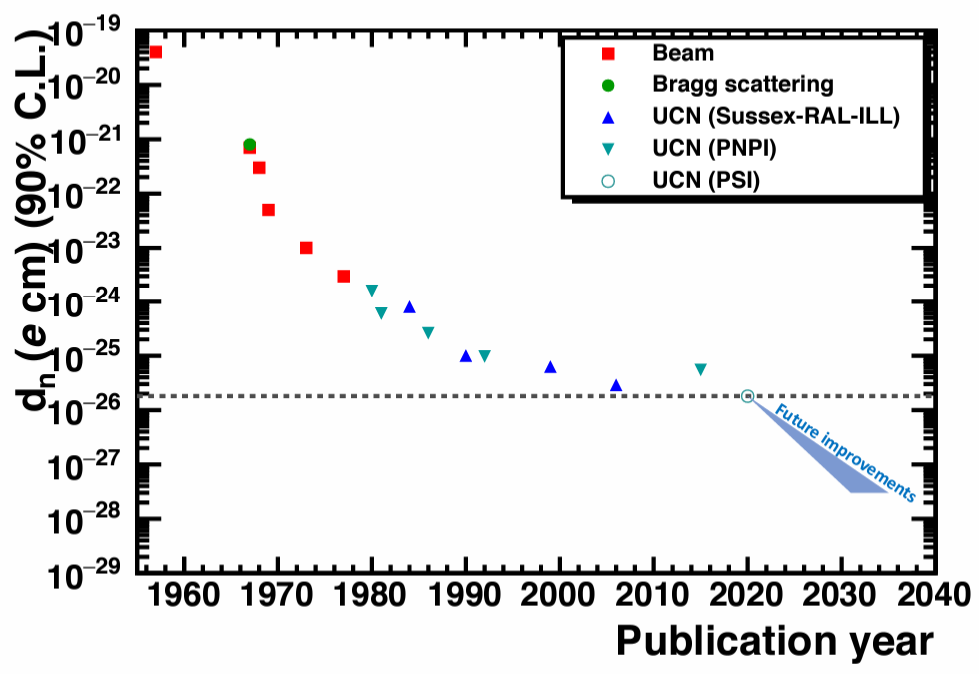
\includegraphics[width=0.5\linewidth]{Snowmass_fig.png}
    \caption{nEDM experimental progress~\cite{Snow22}}
    \label{fig:snowmass}
\end{figure}

% nEDM fixed rho_uu
\begin{figure}[p]
    \centering
    \begin{minipage}{0.48\textwidth}
      \centering
      \includegraphics[width=0.85\linewidth]{example-image}
      \caption{nEDM results.}
      \label{fig:nEDM-fixed}
    \end{minipage}\hfill
    \begin{minipage}{0.48\textwidth}
      \centering
      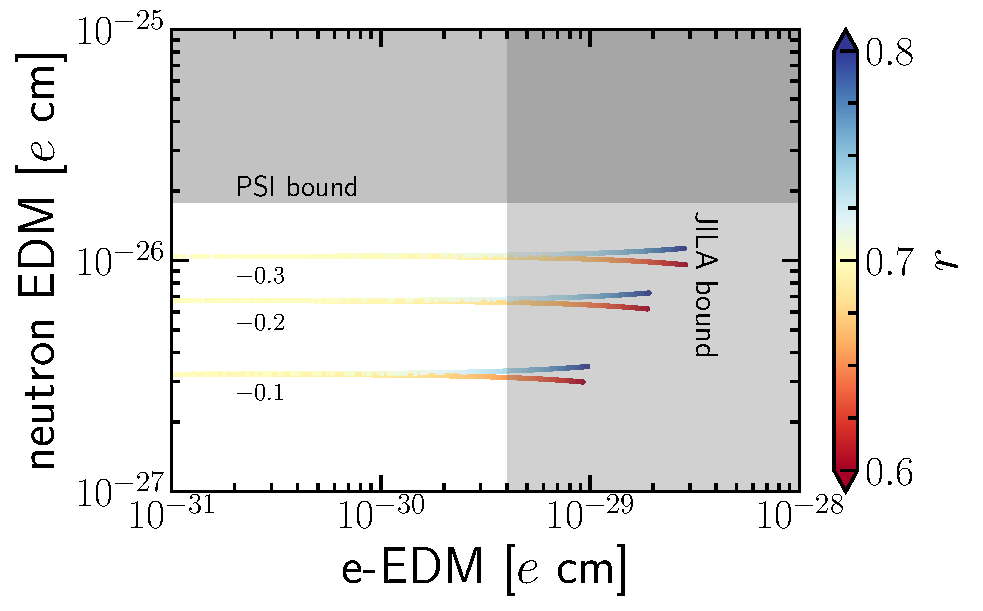
\includegraphics[width=0.95\linewidth]{fig3.pdf}
      \caption{Combined eEDM-nEDM result.}
      \label{fig:nEDM-eEDM}
    \end{minipage}
\end{figure}

% nEDM varying rho_uu
\begin{figure}[p]
    \centering
    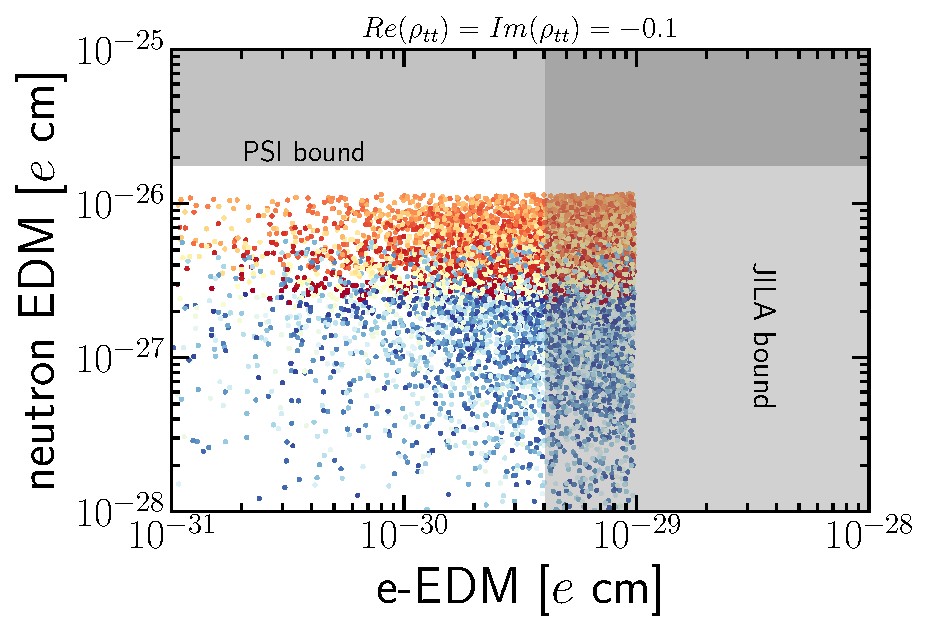
\includegraphics[width=7.35cm,height=5.55cm,angle=-90]{fig4_1.pdf}\\
    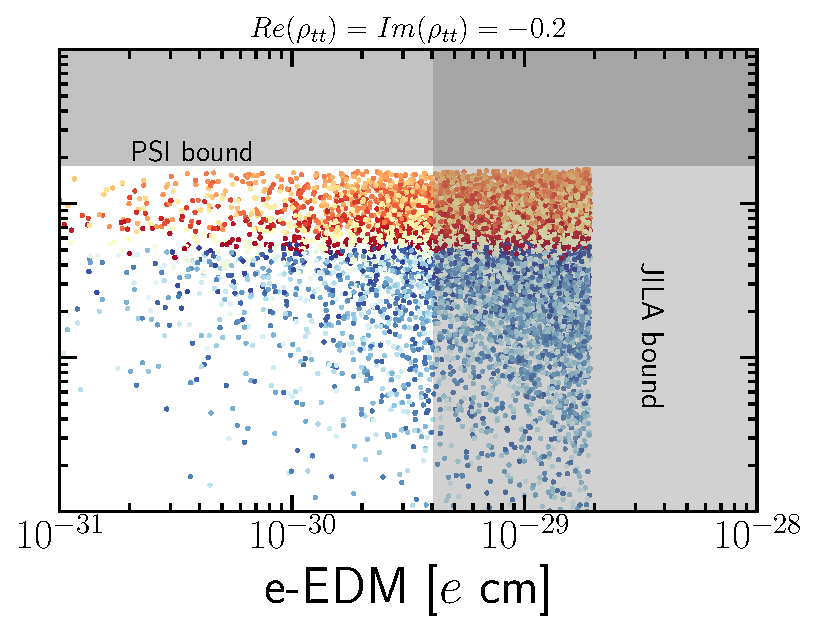
\includegraphics[width=6.45cm,height=5.55cm,angle=-90]{fig4_2.pdf}\\
    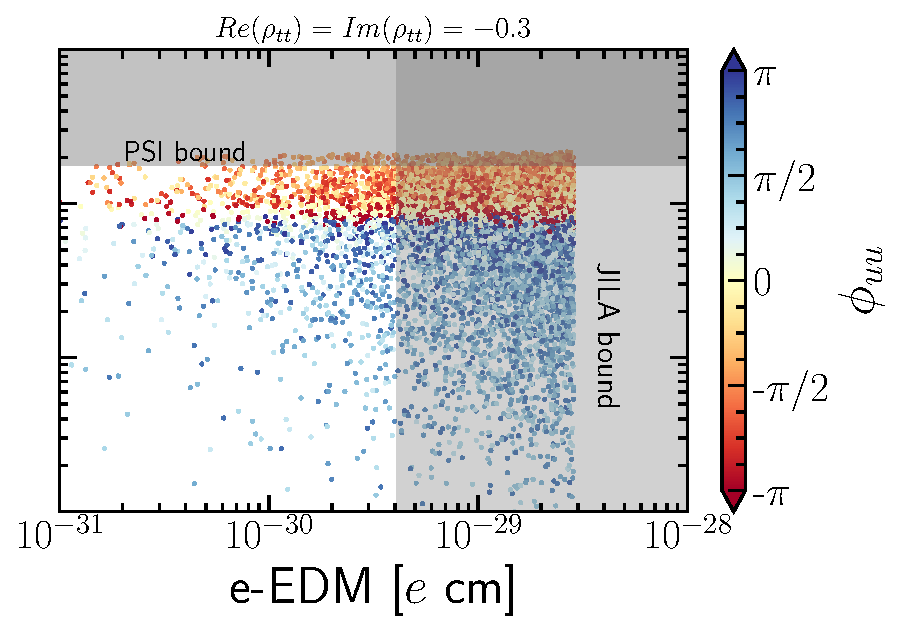
\includegraphics[width=7.89cm,height=5.55cm,angle=-90]{fig4_3.pdf}
    \caption{Results for eEDM and nEDM with \(|\rho_{uu}| \sim \lambda_{u}\).}
    \label{fig:nEDM-varied}
\end{figure}